\subsection{Versuchsaufbau}

\begin{figure}[H]
\begin{center}
  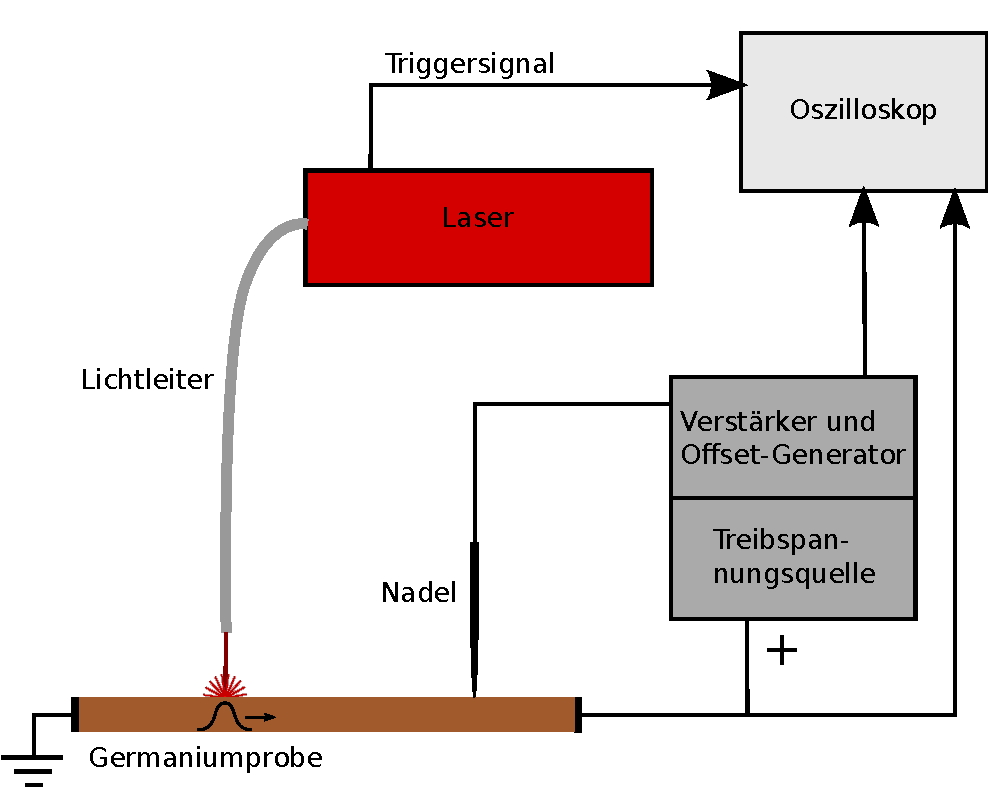
\includegraphics[width=0.75\textwidth]{../img/aufbauHS.pdf}
  \caption{Aufbau für das Haynes-Shockley-Experiment zur Messung der Drift, Diffusion und Rekombination einer
  Elektronenwolke, die von einem Laserpuls erzeugt wird.}
  \label{img:aufbauHS}
\end{center}
\end{figure}

\autoref{img:aufbauHS} zeigt den Aufbau, der beim Haynes-Shockley-Experiment verwendet wird.
Ein Infrarotlaser erzeugt einen kurzen Puls, der über einen Lichtleiter auf die Germaniumprobe fällt.
Dort erzeugt die so zugeführte Energie eine Elektronenwolke,
die sich dann aufgrund einer angelegten Treibspannung in Richtung des höheren Potentials zu einer Nadel bewegt.
Das Spannungssignal der Nadel wird verstärkt,
mit einem Offset versehen, der das Potential der Treibspannung ausgleicht,
und mit einem Oszilloskop angezeigt.
Auf dem zweiten Kanal des Oszilloskops liegt die Treibspannung.
Um die Laufzeit der Elektronenwolke genau bestimmen zu können,
wird das Oszilloskop auf den Laserpuls getriggert.
Da die Germaniumprobe empfindlich auf Erwärmung reagiert,
ist die Treibspannung mit 30\,Hz und einer Pulsweite von 500\,\textmu s gepulst. 
Die Daten des Oszilloskops können auf einem USB-Stick gespeichert werden.